\scanpage{15}
\mspage{4}

Quand il y en a un, l'autre vis de $D\setminus\{\unsure{a|s}\}$ reste libre pour \deleted{\unsure{encore}} être base de triangles de spécialisation pour $D$ (il y en a deux sur la figure ci-dessus). L'ennui, c'est que les \deleted{\unsure{arcs de}}\inserted{\unsure{ou les couloirs de}} spécialisation ne forment pas, avec les autres spéc. et gén. immédiates une structure polygonale \inserted{naturelle}. \deleted{Mais}
\margin{\unsure{mais?} cf plus bas}
\deleted{si $D$ est orienté ou pas}

Peut-être est-il plus instructif de partir de $\Delta$, et regarder l'ens. de ce qu'il convient d'appeler les ``générisations'' \inserted{(immédiates)}. J'en vois de deux

\figure{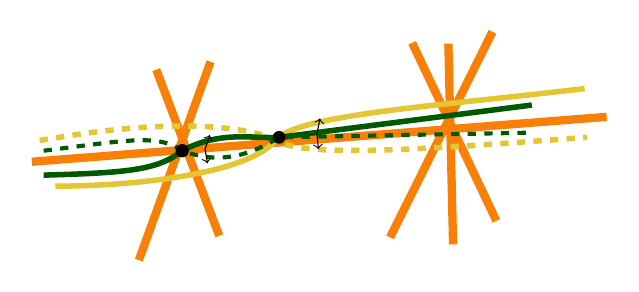
\begin{tikzpicture}[x=1cm,y=1cm]
\draw[orange!90!brown,line width=3pt] (-2.6,-.17)--(4.7,.40);
\draw[orange!90!brown,line width=3pt] (-1.02,1.00)--(-.22,-1.11) (-.33,1.10)--(-1.24,-1.42);
\draw[orange!90!brown,line width=3pt] (2.23,1.34)--(3.30,-.92) (2.69,1.33)--(2.75,-1.22) (3.25,1.48)--(1.95,-1.13);
\draw[yellow!55!brown,line width=2pt] (-2.30,-.48) .. controls(-1.2,-.48) and(.2,-.30)..(.50,.11) .. controls(.80,.43) and (2.5,.53)..(4.42,.76);
\draw[yellow!55!brown,line width=2pt,dashed] (-2.5,.10) .. controls(-.8,.40) and(.1,.28)..(.50,.11) .. controls(.8,-.15) and(2.8,.02)..(4.45,.14);
\draw[green!35!black,line width=2pt] (-2.45,-.34) .. controls(-1.4,-.31) and(-1.0,-.28)..(-.69,-.03) .. controls(-.2,.23) and(.2,.12)..(.54,.14) --(3.75,.55);
\draw[green!35!black,line width=1.5pt,dashed] (-2.45,-.03) .. controls(-1.4,.10) and(-1.0,.19)..(-.69,-.03) .. controls(-.2,-.22) and(.2,-.07)..(.54,.14)--(3.77,.20);
\fill (-.69,-.03) circle(2.4pt);\fill (.54,.14) circle(2.3pt);
\draw[->,thin] (-.40,-.01)--(-.34,.17);\draw[->,thin] (-.40,-.01)--(-.37,-.19);
\draw[->,thin] (1.02,.18)--(1.06,.38);\draw[->,thin] (1.02,.18)--(1.04,-.01);
\end{tikzpicture}}

types, \uline{les stables}, \deleted{et les sous-stables}. Pour les stables, j'en vois deux pour chaque côté, correspondant aux $2$ orientations superficielles le long de l'arête.

\margin{les stables ne sont pas des gén. \uline{immédiates} pourtant, \unsure{ces gén. se} \uline{factorisent} par les sous stables}

Pour les sous-stables, j'en vois également deux pour chaque sommet, correspondant aux deux orientations de $X$ en ce sommet. Ainsi l'ens des \deleted{\unsure{vis}} générisations correspond à l'ens des sommets et des arêtes \unsure{de ce vrai} polygône topologique, image inverse de $\Delta$ dans $\widetilde X$. On fera attention que ce polygône n'est \unsure{\uline{pas}|\deleted{pas}} canoniquement isom. au polygône des vis qu'on avait regardé pour les p.r. $D$ non supercritiques --- le choix d'un isom. dépend du choix d'une orientation de $\Delta$. Tjrs est-il que si $\nu$ est le nb de sommets de $\Delta$, l'ens des générisations \inserted{immédiates} de $\Delta$ s'identifie aux sommets d'un \deleted{\unsure{ens.}} polygône \unsure{croisé} d'ordre \uline{$2\nu+2\nu=4\nu$}$^*$, rev. d'ordre $2$ du collier défini par $\Delta$. L'une des orientations de ce polygône est liée donc à l'une des orientations de $\Delta$ lui-$=$.

\margin{$^*$ ou, d'ordre $2\nu$ seulement en se bornant aux gén. \uline{immédiates}}
\margin{14}
